\subsection{Aufgabe 11}

Mit Hilfe des Oszilloskops konnten wir sehr schön die erwartete Gaußkurve sehen und vermessen. Außerdem entdeckten wir den ''power dip'', der in der Mitte der Gaußkurve auftauchte und ungefähr Halbwertshöhe annahm. 

\begin{figure}[here]
\centering
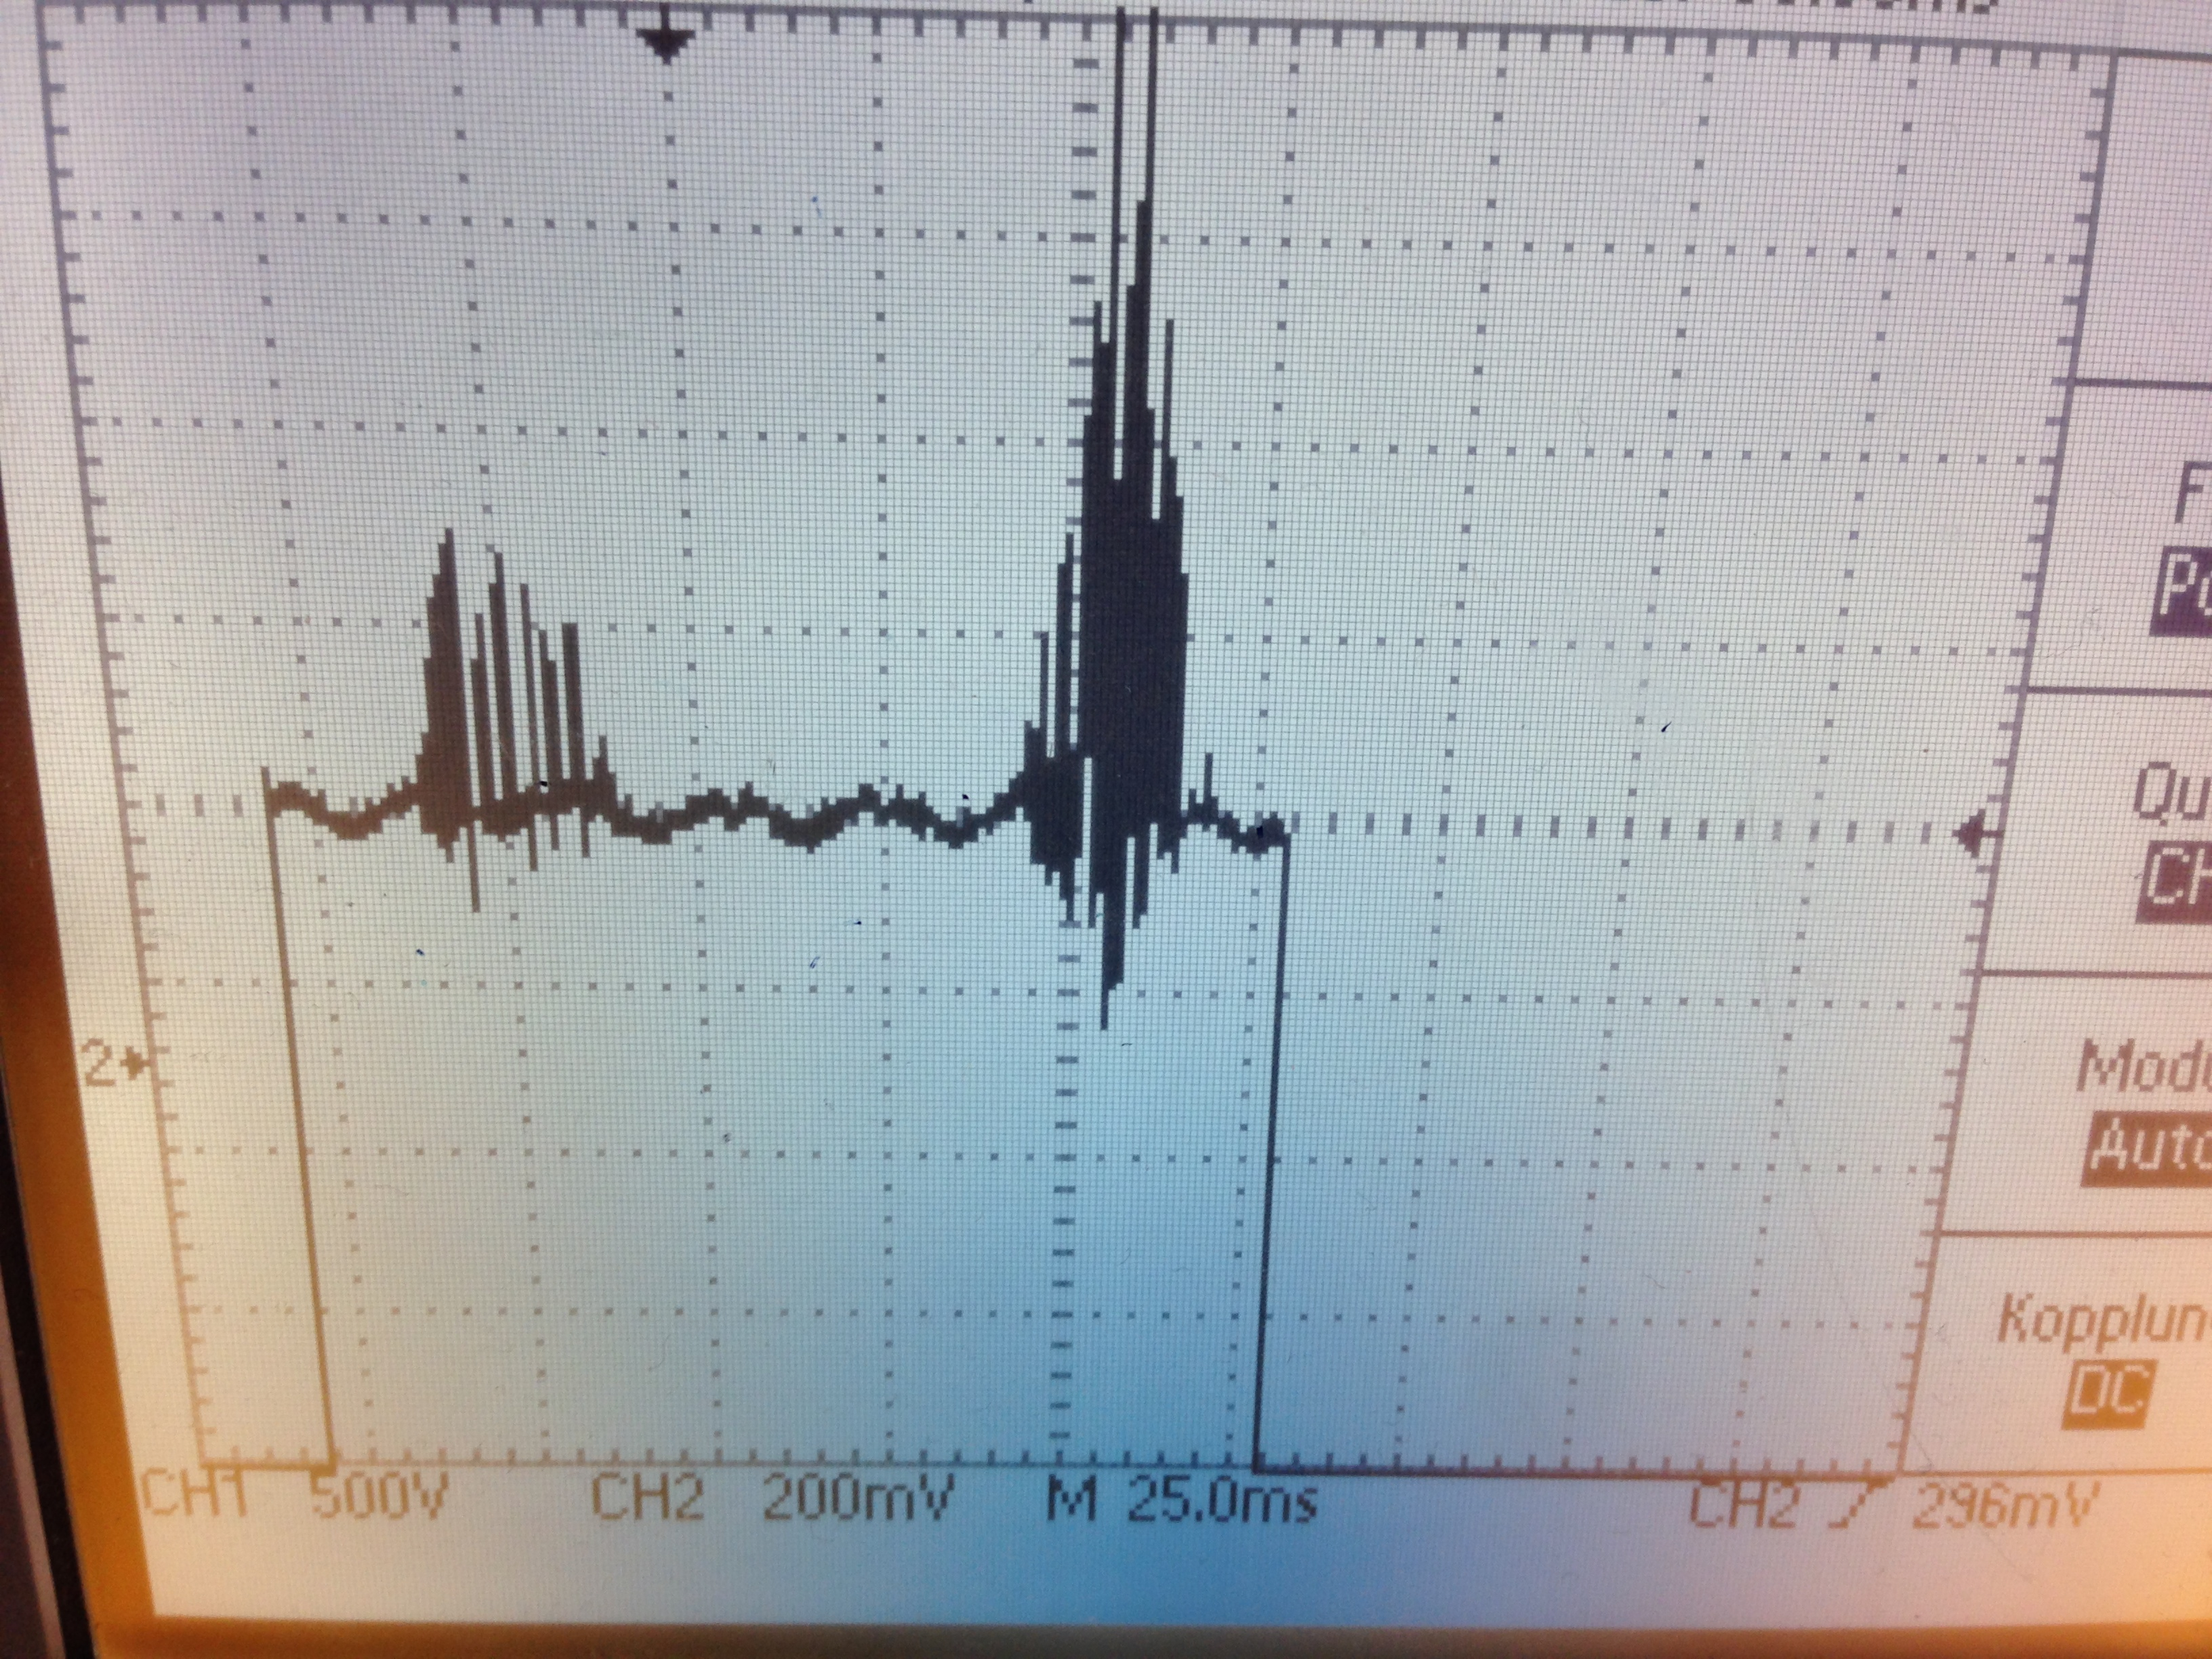
\includegraphics[scale=0.1]{img/62}
\caption{Power-Dips}
\begin{center}
\end{center}
\end{figure}

Wie in Abb. 4 dargestellt, sind nur einige Moden in einer Gaußkurve zu sehen. Wir haben diese ungefähr verlaufende Kurve zur genaueren Bestimmung der Halbwertsbreite vermessen. Wir erhielten eine Breite von (0.600 $\pm$ 0.050) GHz. Setzen wir diese in Gleichung (12) zusammen mit der Masse der Neon-Atome von m = 3.35*10$^{26}$ kg und der Frequenz des Lasers von $\nu$ = 633 nm ein, so erhalten wir eine Temperatur von ca. 63.14 K. Dieser Wert ist offensichtlich unrealistisch gering. Wir sehen also, dass unsere Abschätzung der Halbwertshöhe anhand der Gaußkurve immer noch nicht gut genug war.
